\documentclass{article}

\usepackage{polski}
\usepackage[utf8]{inputenc}
\usepackage{graphicx}
\usepackage{float}
\usepackage{amsmath}
\usepackage{geometry} 

\author{Jakub Postępski}
\title{MODI, projekt 2, zadanie 33}
\begin{document}
\maketitle
\section{Identyfikacja modeli statycznych}
Wykorzystano dane statyczne dla zestawu 33 (rysunek \ref{fig:danestatyczne}).
\begin{figure}
\centering
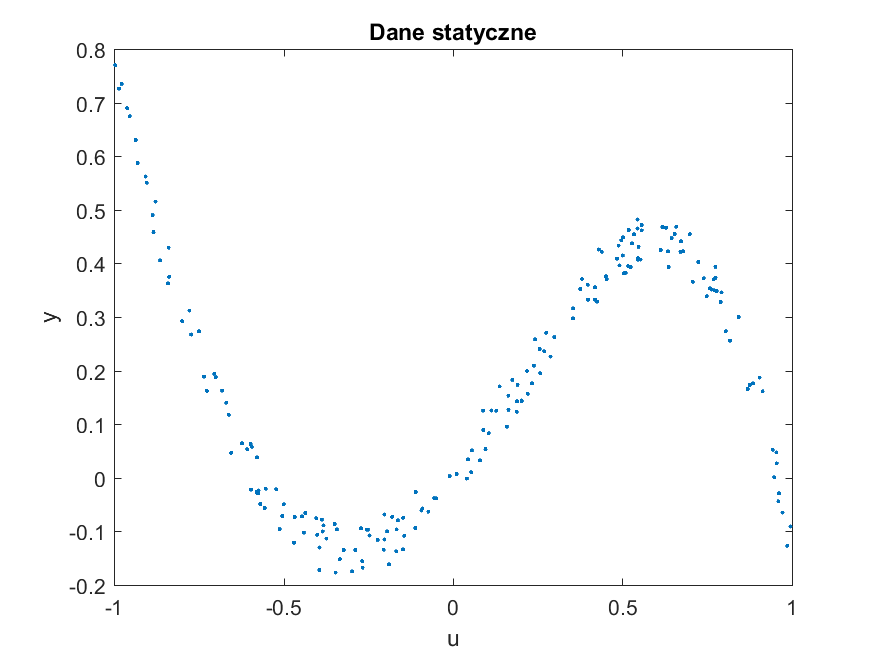
\includegraphics[width=0.95\linewidth]{dane_statyczne}
\caption{Dane statyczne}
\label{fig:danestatyczne}
\end{figure}

Podzielono dane statyczne na zbiór uczący (rysunek \ref{fig:danestatyczneuczace}) oraz zbiór weryfikujący (rysunek \ref{fig:danestatyczneweryf}), poprzez przypisanie każdego kolejnego elementu danych statycznych do innego zbioru.\\
Wyznaczono statyczne modele nieliniowe postaci
\[y(u) = \sum_{i = 0}^{N}a_i u^i\]

\begin{tabular}{|c|c|c|c|c|c|c|c|c|c|}
\hline 
$N$ & $a_0$ & $a_1$ & $a_2$ & $a_3$ & $a_4$ & $a_5$ & $a_6$ & $E_{ucz}$ & $E_{wer}$ \\ 
\hline 
1 & 0.1806 & 0.0519 & - & - & - & - & - & 0.12872 & 0.0021702 \\ 
\hline 
2 & 0.0447 & 0.0517 & 0.4014 & - & - & - & - & 0.37595 & 0.024406 \\ 
\hline 
3 & 0.0467 &  0.7964&0.3795  &-1.2511  & - & - &-  &0.016417  &0.00019188  \\ 
\hline 
4 & -0.0048 & 0.7935 & 0.8324 & -1.2540  & -0.5050 & - & - & 0.0011411 & 0.00012017 \\ 
\hline 
5 &-0.0049  & 0.8033 & 0.8340 &   -1.2987&  -0.5066& 0.0389 & - & 0.0013553 & 8.5264e-05 \\ 
\hline 
6 & -0.0033 &  0.8037&  0.8039& -1.3017 &-0.4171  &0.0418  & -0.0645 & 0.0012089 & 8.4509e-05 \\ 
\hline 

\end{tabular} 
Należy zaznaczyć, że w tabelce opisany jest też model rzędu pierwszego, czyli model liniowy, z podpunktu c).\\
Osiągnięta sytuacja jest dość nietypowa, bo dane weryfikujące mają mniejszy błąd niż dane uczące.\\
Według autora najlepszym wyborem jest model z wielomianem stopnia 4. Nie ma on wiele większych błędów niż inne modele i jest stosunkowo prosty.
\begin{figure}
\centering
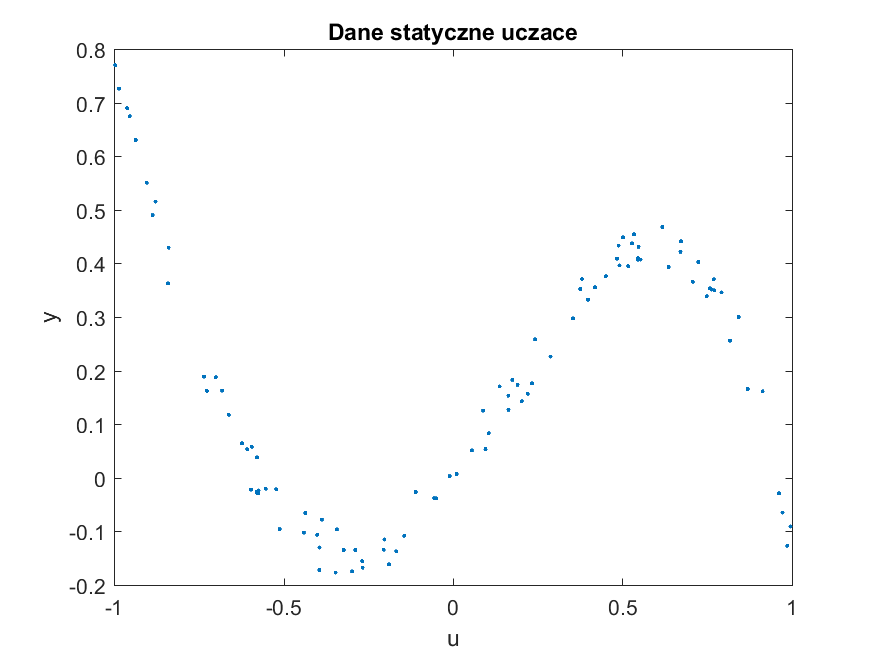
\includegraphics[width=0.95\linewidth]{dane_statyczne_uczace}
\caption{Dane statyczne, zbiór uczący}
\label{fig:danestatyczneuczace}
\end{figure}

\begin{figure}
\centering
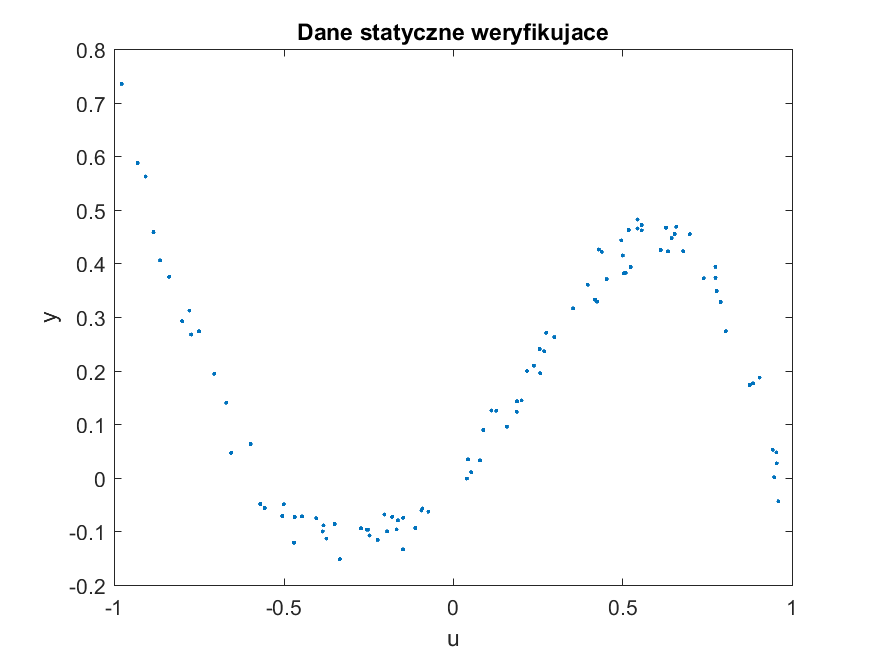
\includegraphics[width=0.95\linewidth]{dane_statyczne_weryf}
\caption{Dane statyczne, zbiór weryfikujący}
\label{fig:danestatyczneweryf}
\end{figure}

\begin{figure}
\centering
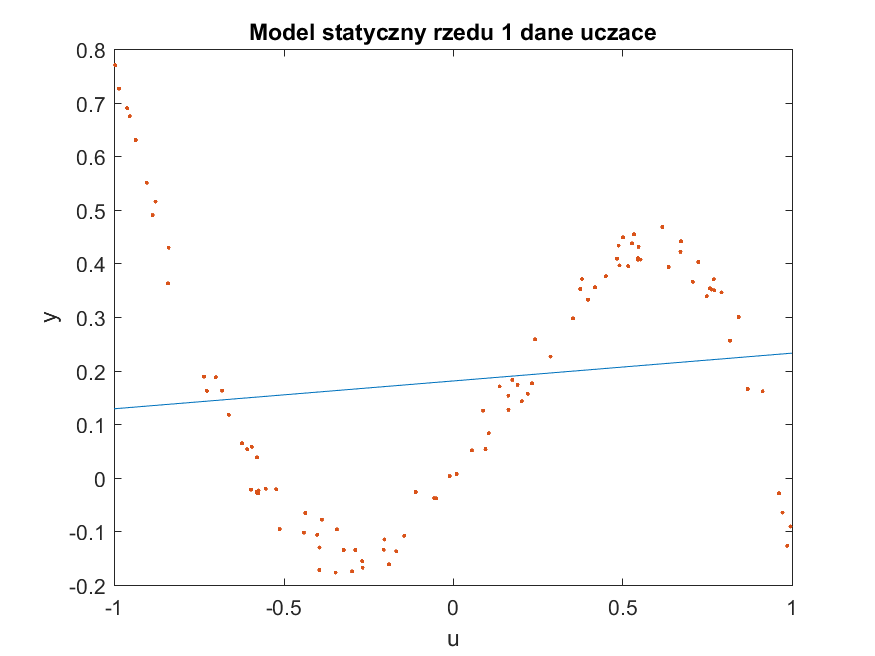
\includegraphics[width=0.95\linewidth]{dane_statyczne_model_rzedu_1_uczace}
\caption{Dane statyczne(uczące) i model dla wielomianu stopnia 1}
\label{fig:danestatyczneuczace1}
\end{figure}

\begin{figure}
\centering
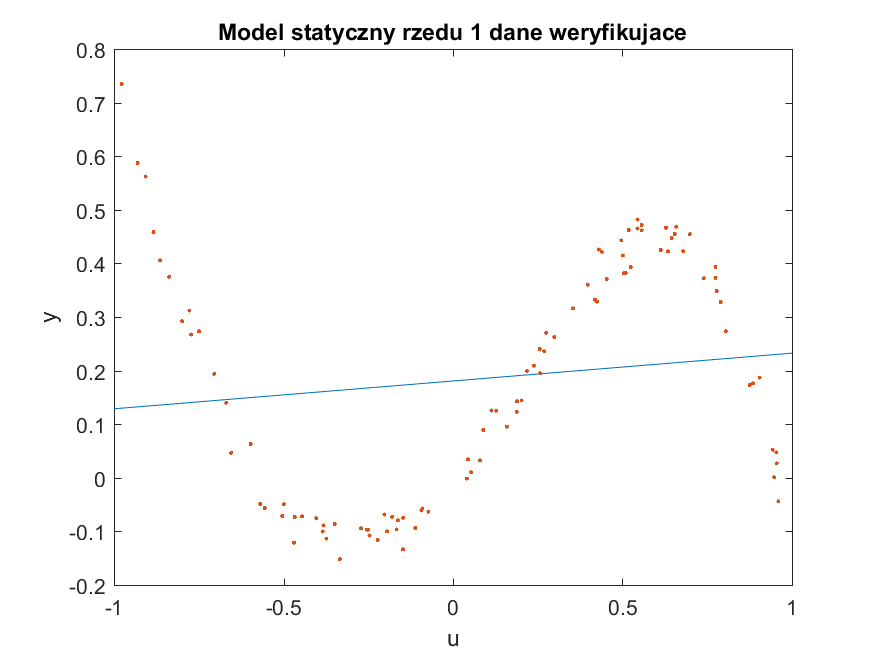
\includegraphics[width=0.95\linewidth]{dane_statyczne_model_rzedu_1_weryf}
\caption{Dane statyczne(weryfikujące) i model dla wielomianu stopnia 1}
\label{fig:danestatyczneweryf1}
\end{figure}

\begin{figure}
\centering
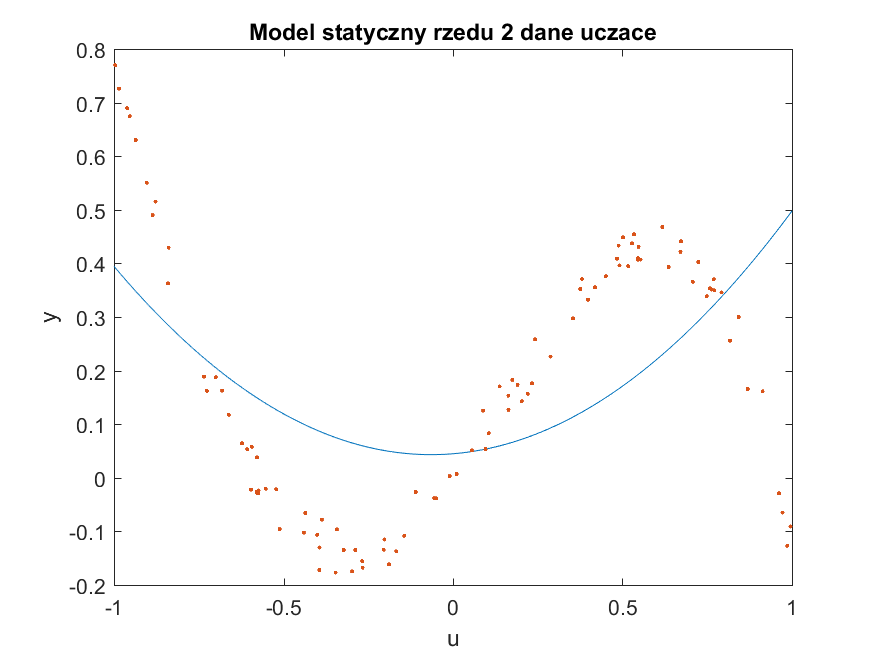
\includegraphics[width=0.95\linewidth]{dane_statyczne_model_rzedu_2_uczace}
\caption{Dane statyczne(uczące) i model dla wielomianu stopnia 2}
\label{fig:danestatyczneuczace2}
\end{figure}

\begin{figure}
\centering
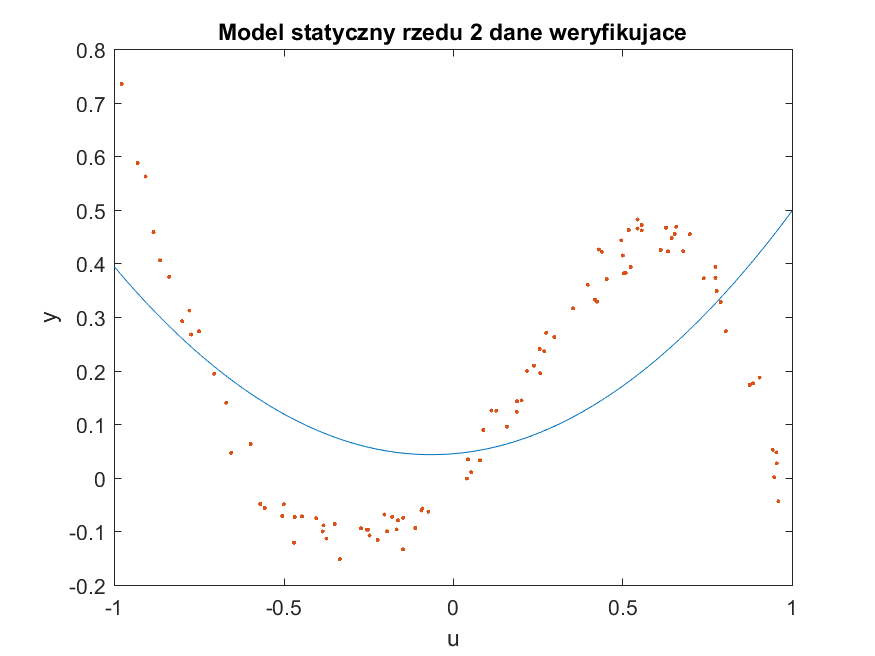
\includegraphics[width=0.95\linewidth]{dane_statyczne_model_rzedu_2_weryf}
\caption{Dane statyczne(weryfikujące) i model dla wielomianu stopnia 2}
\label{fig:danestatyczneweryf2}
\end{figure}

\begin{figure}
\centering
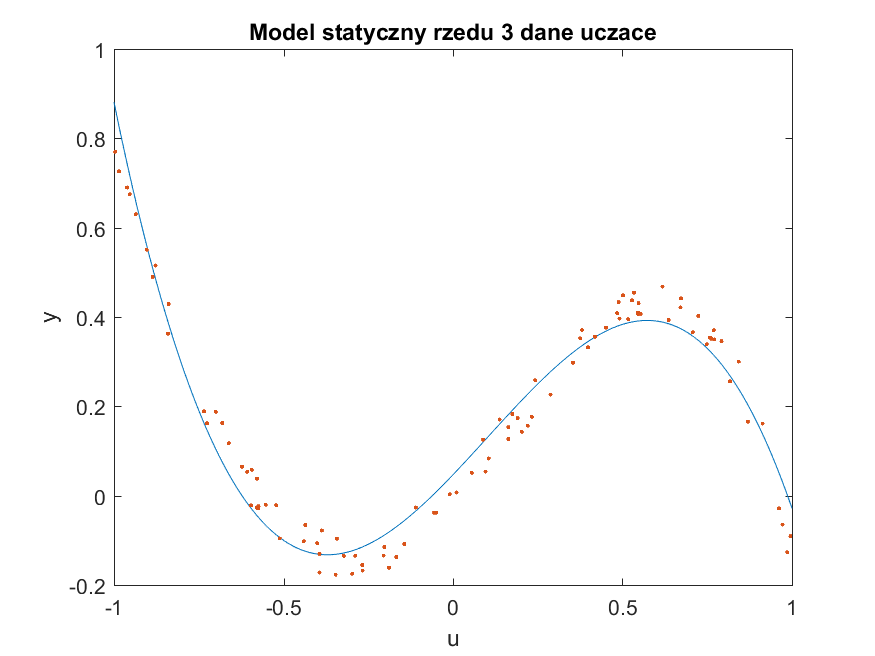
\includegraphics[width=0.95\linewidth]{dane_statyczne_model_rzedu_3_uczace}
\caption{Dane statyczne(uczące) i model dla wielomianu stopnia 3}
\label{fig:danestatyczneuczace3}
\end{figure}

\begin{figure}
\centering
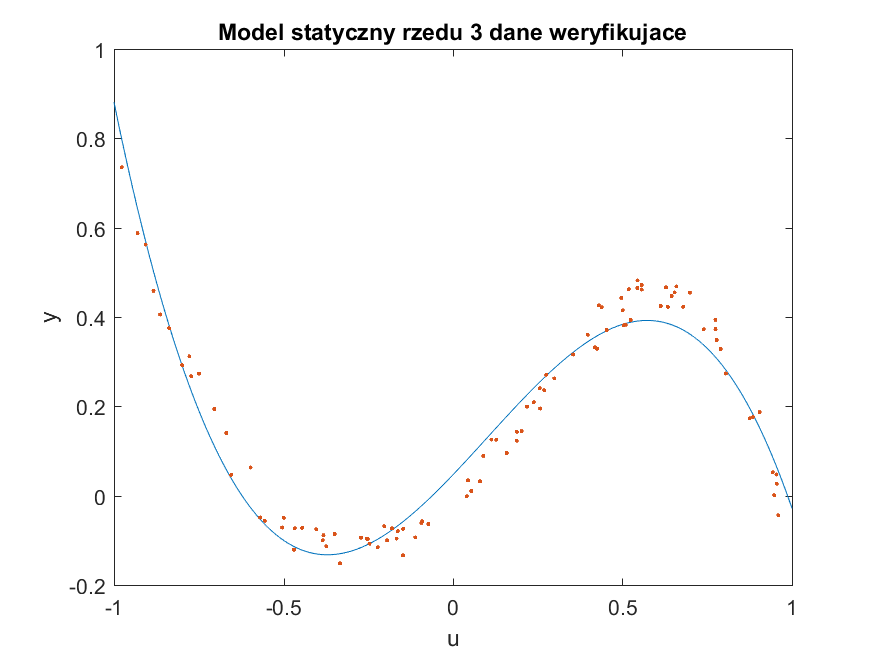
\includegraphics[width=0.95\linewidth]{dane_statyczne_model_rzedu_3_weryf}
\caption{Dane statyczne(weryfikujące) i model dla wielomianu stopnia 3}
\label{fig:danestatyczneweryf3}
\end{figure}

\begin{figure}
\centering
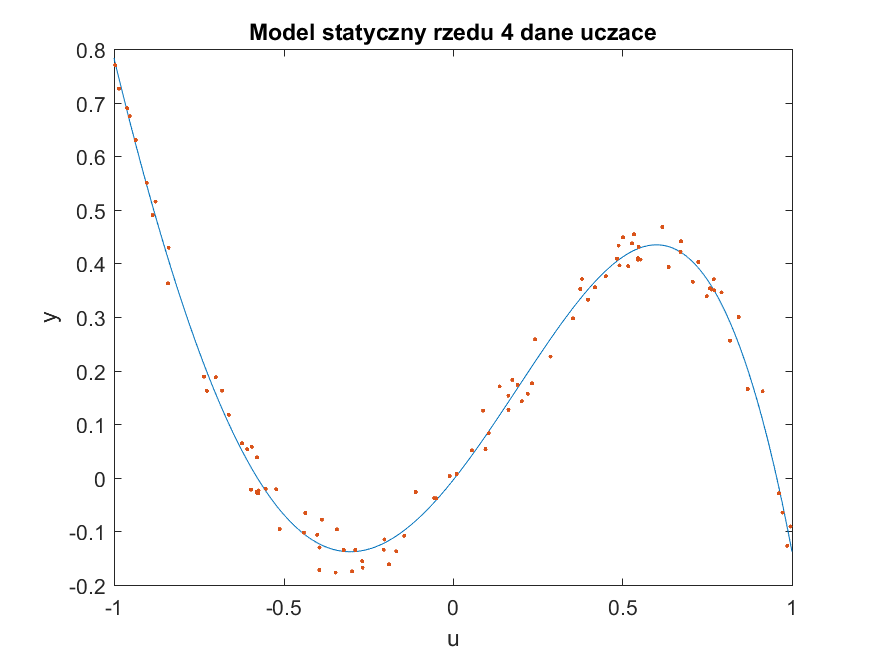
\includegraphics[width=0.95\linewidth]{dane_statyczne_model_rzedu_4_uczace}
\caption{Dane statyczne(uczące) i model dla wielomianu stopnia 4}
\label{fig:danestatyczneuczace4}
\end{figure}

\begin{figure}
\centering
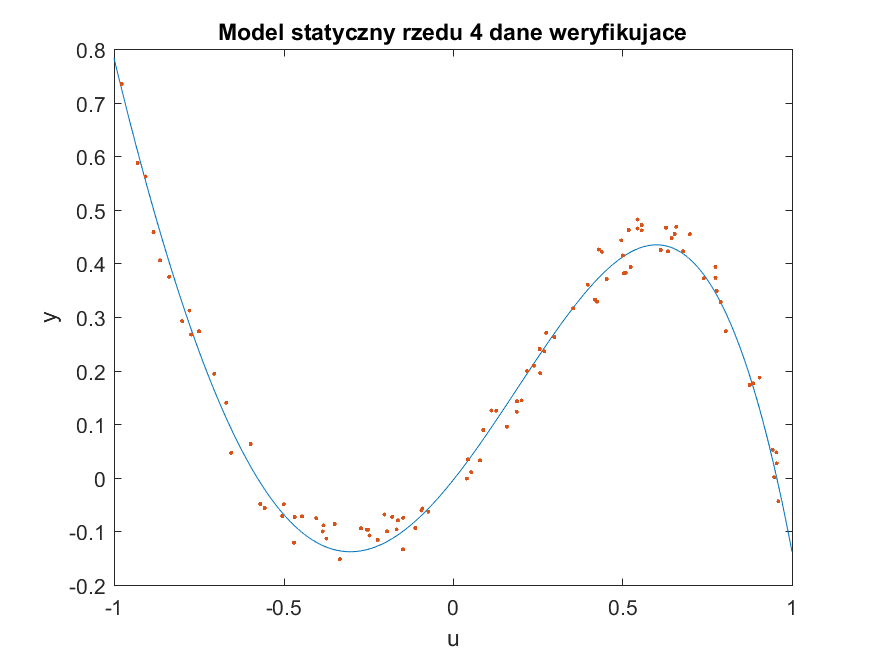
\includegraphics[width=0.95\linewidth]{dane_statyczne_model_rzedu_4_weryf}
\caption{Dane statyczne(weryfikujące) i model dla wielomianu stopnia 4}
\label{fig:danestatyczneweryf4}
\end{figure}

\begin{figure}
\centering
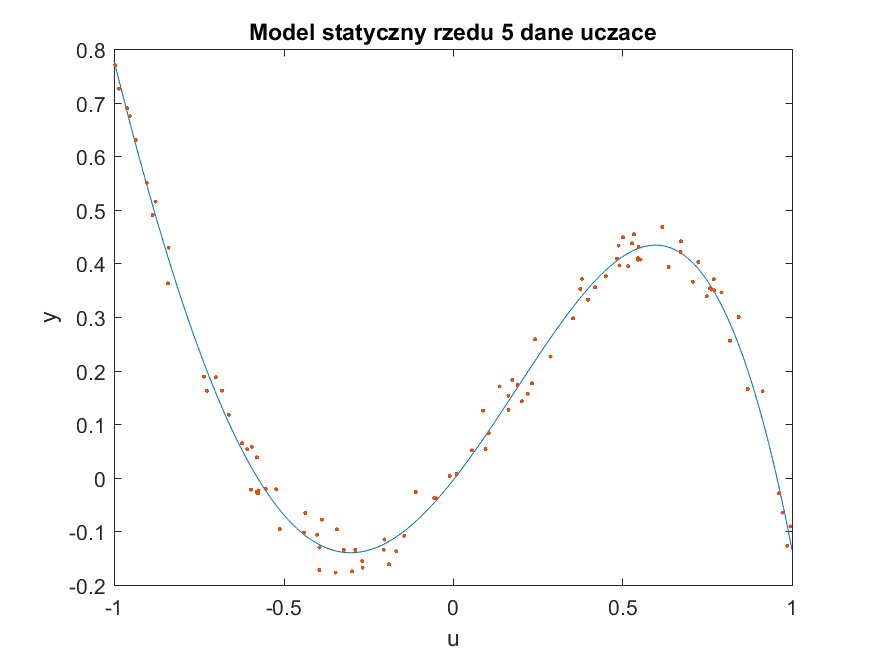
\includegraphics[width=0.95\linewidth]{dane_statyczne_model_rzedu_5_uczace}
\caption{Dane statyczne(uczące) i model dla wielomianu stopnia 5}
\label{fig:danestatyczneuczace5}
\end{figure}

\begin{figure}
\centering
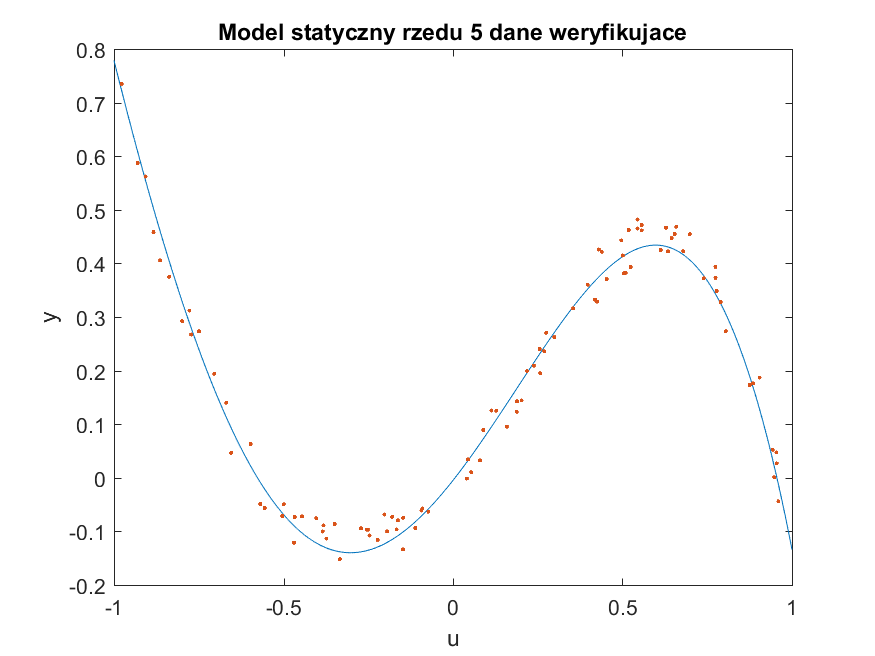
\includegraphics[width=0.95\linewidth]{dane_statyczne_model_rzedu_5_weryf}
\caption{Dane statyczne(weryfikujące) i model dla wielomianu stopnia 5}
\label{fig:danestatyczneweryf5}
\end{figure}

\begin{figure}
\centering
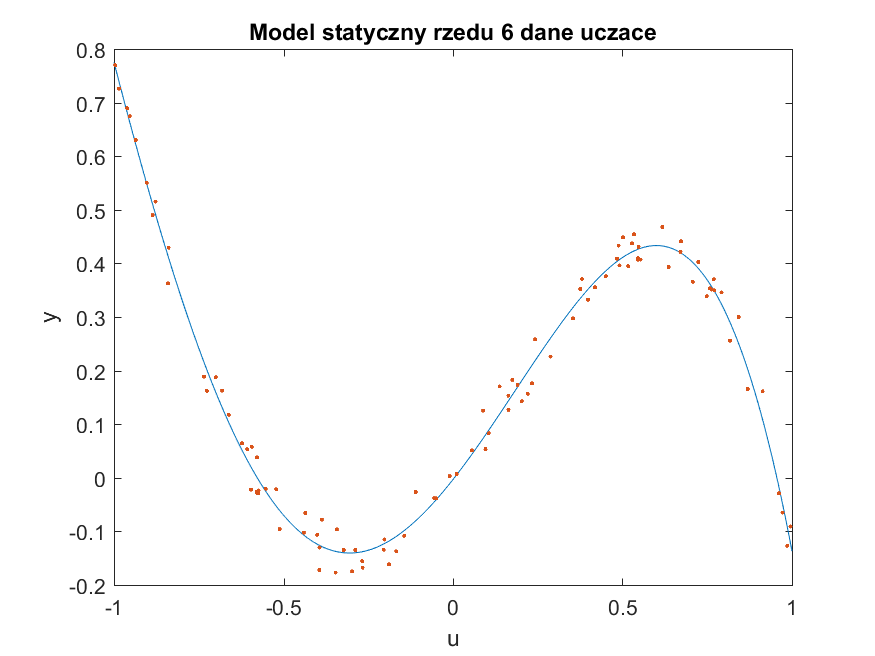
\includegraphics[width=0.95\linewidth]{dane_statyczne_model_rzedu_6_uczace}
\caption{Dane statyczne(uczące) i model dla wielomianu stopnia 6}
\label{fig:danestatyczneuczace3}
\end{figure}

\begin{figure}
\centering
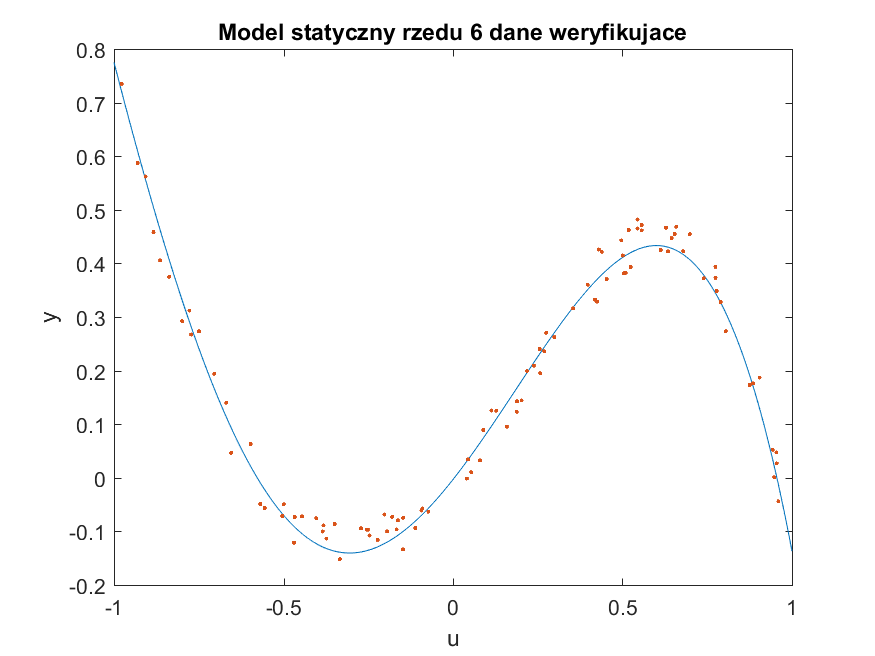
\includegraphics[width=0.95\linewidth]{dane_statyczne_model_rzedu_6_weryf}
\caption{Dane statyczne(weryfikujące) i model dla wielomianu stopnia 6}
\label{fig:danestatyczneweryf6}
\end{figure}

\end{document}
